\documentclass{standalone}

\usepackage{tikz}
\usetikzlibrary{calc,positioning,decorations.markings}
\begin{document}

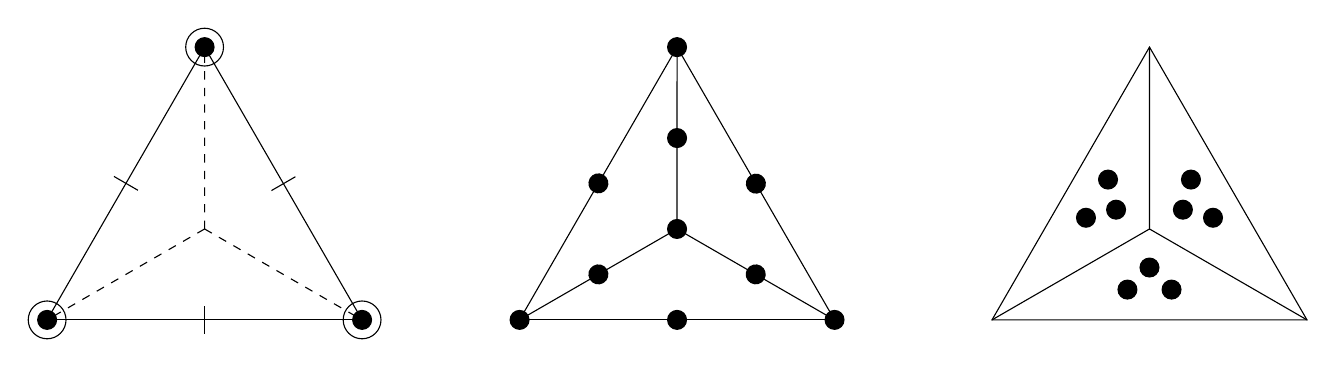
\begin{tikzpicture}[scale=4,
    normaldofs/.style={postaction=decorate, decoration={markings, mark=at position 0.5 with {
            \draw (0,-5pt) -- ++(0, 10pt);
    }}},
    pointdofs/.style={postaction=decorate, decoration={markings, mark=at position 0.5 with {
                \draw [fill] circle (0.12);
    }}}
    ]
    \coordinate (0) at (0, 0) {};
    \coordinate (1) at (1, 0) {};
    \coordinate (2) at ($(0) + (60:1)$) {};
    \coordinate (bc) at (barycentric cs:0=1,1=1,2=1) {};

    \draw[normaldofs] (0) to (1);
    \draw[normaldofs] (1) to (2);
    \draw[normaldofs] (2) to (0);

    \foreach \i in {0, 1, 2} {
        \draw (\i) circle (0.06);
        \draw[fill] (\i) circle (0.03);
    }

    \foreach \i in {0, 1, 2} {
        \draw[dashed] (bc) -- (\i);
    }
    \begin{scope}[shift={(1.5, 0)}]

        \coordinate (0) at (0, 0) {};
        \coordinate (1) at (1, 0) {};
        \coordinate (2) at ($(0) + (60:1)$) {};
        \coordinate (bc) at (barycentric cs:0=1,1=1,2=1) {};

        \draw[pointdofs] (0) to (1);
        \draw[pointdofs] (1) to (2);
        \draw[pointdofs] (2) to (0);
        \foreach \i in {0, 1, 2} {
            \draw[pointdofs] (bc) -- (\i);
        }

        \foreach \i in {0, 1, 2} {
            \draw[fill] (\i) circle (0.03);
        }

        \draw[fill] (bc) circle (0.03);
    \end{scope}
    \begin{scope}[shift={(3, 0)}]
        \coordinate (0) at (0, 0) {};
        \coordinate (1) at (1, 0) {};
        \coordinate (2) at ($(0) + (60:1)$) {};
        \coordinate (bc) at (barycentric cs:0=1,1=1,2=1) {};
        \draw[line join=miter] (0) -- (1) -- (2) -- cycle;
        \draw[line join=miter] (0) -- (bc) -- (1);
        \draw[line join=miter] (2) -- (bc);

        \coordinate (bc0) at (barycentric cs:0=1,1=1,bc=1) {};
        \coordinate (bc1) at (barycentric cs:1=1,2=1,bc=1) {};
        \coordinate (bc2) at (barycentric cs:0=1,2=1,bc=1) {};

        \foreach \i in {0, 1, 2} {
            \draw[fill] ($(bc\i)-(\i*120 + 0:0.07)$) circle (0.03);
            \draw[fill] ($(bc\i)+(\i*120 + 0:0.07)$) circle (0.03);
            \draw[fill] ($(bc\i)+(\i*120 + 90:0.07)$) circle (0.03);
        }
    \end{scope}
\end{tikzpicture}

\end{document}
